\documentclass[12pt]{article}
\usepackage[onehalfspacing]{setspace}
\usepackage{amsmath, bm, graphicx}
\newcommand{\myfont}{\fontfamily{pcr}\selectfont}
\usepackage[margin=1in]{geometry}
\usepackage[parfill]{parskip}
%\usepackage[none]{hyphenat}
\usepackage[usenames]{xcolor}
\graphicspath{{./plots/}}


\newcommand{\thanh}[1]{{\color{blue} [Thanh: #1]}}

\title{Kaggle Project Report \\ Team name: NotTooDeep\_Learning}
\author{Ben Buzzee, Thanh Nguyen, Kellie McClernon}

\begin{document}
\maketitle


\textbf{Final Scores}
\begin{center}
\begin{tabular}{l c c}
	\hline
	Model & Test Error (Public) & Full Test Error (Private) \\
	\hline
	Ensemble of PLS, Neural Net, and Xgboost & 0.115738 & 0.119502 \\
	Ensemble of PLS and Xgboost & 0.117672 & 0.123988 \\
	\hline
\end{tabular}
\end{center}

\begin{center}
\begin{tabular}{l c c}
	\hline
	Model & CV Error & Test Error\\
	\hline
	PLS & 0.114 & 0.1205 \\
	Deep Neural Net & 0.094 & 0.1267 \\
	\hline
\end{tabular}
\end{center}


\section{Initial Model Fitting}

We initially reviewed the data to become familiar with the data types, number of categorical variables, how granular the categorical variables were, and where there were missing values. \thanh{Knowing that over 50\% of the predictors are categorical, we aimed for random forest to take advantage of its scale invariant property. We also fitted some linear methods on data with only numerical variables to get intial ideas and establish a baseline.}  %Despite the missing values, we wanted to fit some initial models to establish a baseline, but 
We then learned that most methods cannot handle missing values and that caret will often throw out all cases with NA before fitting while more than half of the data cases included missing values. %This would result in a major loss of information.  
Therefore, we spent the first weeks pre-processing the data, trying to familiarize with the data and reduce the number of missing values.

Starting from the data description, we realized that some NA's were not representing missing values but rather an extra category of ``none" or zero.  For example, the variable ``Pool Quality" had NA's for more than 90\% of the data.  However ``Pool Quality" was missing not because it was unobserved when there was in fact a pool, but instead because no pool was present.  This case is different than missing at random.  Therefore we replaced NA's for these types of categories with "None".  For numerical predictors such as ``Pool" square feet and ``Garage" square feet, we replaced the NA with zero.

%Prior to fitting models, we also needed to remove the Id column from the train set since this is not a predictor. 
We noticed that R was importing ``MSSubclass" as a numerical value but actually this was a categorical variable with numerical labels.  Therefore we needed to convert the field to factor so that R would recognize the labels as levels of a category.  Additionally since the test set is validated against $log$ SalePrice based on the instructions from Kaggle, we transformed the response to $\log$ of the sale price.  Note,  we did not need to adjust for zero sale prices since there can not a zero sale value in the data set.

We considered imputation of missing values, such as using random forest to impute values or nearest neighbor.  However, to use random forest imputation, you must grow trees and values are imputed based on proximity. This raises a couple of immediate starting questions, such as how many trees or iterations are optimal.  But then you have to start to wonder about growing trees to impute data values and then growing trees again off the new imputed set, surely this causes some type of self-fulfilling prophesy, especially if your variable \emph{mtry} is too large. We also learned if you want to use cross validation to tune your model parameters, you will run into the issue that you already leveraged your entire data set to impute values so your out-of-bag errors during the cross-validation step will be overly optimistic.  There is a similar issue with nearest neighbor imputation.

Due to GBM explicit handling of NA's without imputation, at this point we choose to fit a model with GBM.  The generalized boosted regression model provided the best repeated cross-validation RMSE at .1307 (for log transformed saleprice). Our submission results were surprisingly similar with a RMSE of 0.13066. % Mention of fitting other models, do we remember which ones?
\thanh{Besides, fitting PCR, Ridge and PLS on the data with numerical variables resulted in cross-validation errors of 0.1412, 0.1427 and 0.1255 respectively.}

\section{Replacing Missing Values}

We still had the issue of missing values where the true value was unknown. Therefore, initially we replaced those missing values with medians for quantitative variables or modes for categorical. We used the entire training data set to find the medians and modes prior to cross validation for our models, which we realized later was data snooping and caused our CV error to be misleading since information about the entire data set is contained in each fold through the imputed median or mode.

At this point we wanted to focus on dimension reduction. To accomplish this, we performed a principal component analysis to see if we could identify some predictors with significantly high eigenvalues. However, most values were very high and fairly close to each other. We suspect this is because of the high correlation among our variables.  Additionally, PCA takes only numerical values. %We learned that if you use caret to accomplish a principal component analysis, caret simply will remove any non-numerical fields and then center and scale the left-over numerical fields. Since we still had a large number of categorical fields, this was a potential issue. \thanh{it's trivial}
Hence, we converted the categorical fields to dummy variables so that they would have a numeric representation. However, we learned that while standardization is necessary for PCA, as well as other methods, when you have indicator variables you lose interpretability when you center to mean zero.  There seem to be two thoughts around this: (1) that it would be best to find another method for indicators but few alternatives suggested, and (2) just necessary to standardize to get information out of PCA, so we should be okay will the loss of interpretability in exchange for the gain of information from PCA.  Our group is undecided since we would like an interpretable model but also we are looking to reduce our number of features

We also tried shrinkage methods such as Lasso and Elastic net as methods of predictor selection because we believed they could select only some important variables to explain the data. Nevertheless, Lasso works for only numerical variables %and has similar issues to PCA notes above.
and have difficulity in fitting as the variables are highly correlated.

We fit a variety of models, such as elastic net, lasso, PLS, and xgboost, mostly linear models.  We noticed that so far, without much feature engineering, all our models have roughly the same CV, around 0.13.  With our first ensemble of three models, all of which had similar error rates of 0.14 to 0.13, we got a CV error rate of about 0.12, which is not a very large improvement. We learned that if all the models have a similar error rate, then ensembling does not give us a very significant lift. Therefore, we wanted to aim to improve our feature selection and approach to non-linear regression models in order to get at least one standalone model with error rate closer to 0.10.

\section{Data Revisited}

Since we tried fitting numerous models and all performed similarily, we hypothesized that the issue might be our data needs further cleaning and we need to think more about new informed features. We now were beginning to see that when fitting models the bulk of the time is actually spent cleaning data because models built on bad data and with poor predictors can not perform well no matter how highly acclaimed your model, such as xgboost and deep neural network, maybe. Methods can not make up for inadequencies in the data it is training on.

We read over some data processing kernels posted on Kaggle and from there borrowed the ideas of converting ordinal categories, such as the quality and condition variables, to numerical ordinal values, i.e. 1 - 5. This seems to have value because it will help for models that depend on numerical inputs only while still maintaining the information in the original data set. Additionally methods such as random forest which are invariant to scale are unaffected by transforming categories to numerical and can gain from the additional information of order that is better represented in the numerical scale. Also, some categories had a lot of granularity which caused there to be few cases in certain categories.  By combining related categories, we could get more cases per categories to help train the model.  

\begin{center}
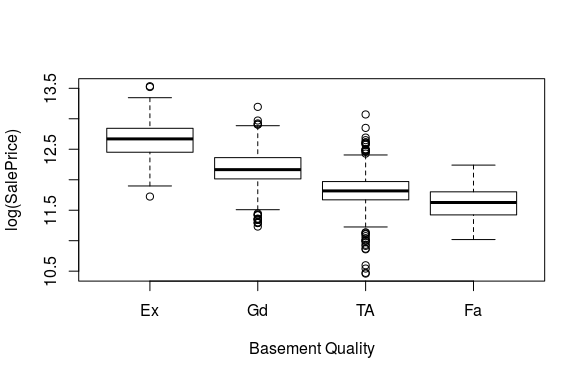
\includegraphics[width = 3in]{bsmtqual.png}
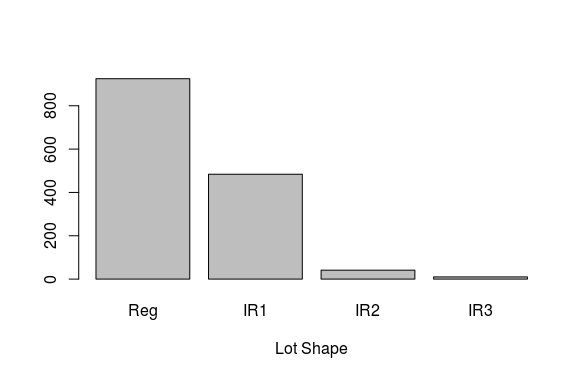
\includegraphics[width = 3in]{lotshape.png}
\end{center}

Further imputation of missing values with the median for numerical values and the mode for categorical were adopted.  We used the whole data set in order to find the medians and mode.  Preferably, we should have calculated the medians and modes for imputation within each fold of our repeated cross-validation step, but due to time constraints and lack of ease for programming, we did the processing before CV.  To use caret's train process with repeated CV, we would have had to write our own method for each model we wanted to fit in order to incorporate our imputation process in each fold.  Since we were interested in several models, this would have been too time consuming.  By taking some samples of 90\% of the training cases and imputing values for the sample, the differences between the samples' imputated values and the ones obtained from the entire set did not seem different enough to warrant the necessity of creating original coding for each model.  (We sampled 90\% of the data to mimic the process of 10-fold CV.)

New features were created such as an indicator for new houses and from the kernels we gathered additional information on the neighborhoods.  Dealing with the neighborhood predictor proved the most challenging because we want to do mappings for geo-location, income, etc.  However, while trying to find information about the neighborhoods, it seemed that these categories are specialized real estate divisions.  A house being in the neighborhood of ``Crawford" means something very specific to a real estate agent, but to the world at large, i.e. what can be found through google, this does not seem the case.  Therefore, we imputed median house price per neighborhood as a proxy for median income.


\section{Choosing Predictors}

On a different data set that only fixed zeros from NA and changed ordinal categorical variables to numerical scale, we saw that the most outstanding issue was Lot Frontage with about 15\% of the data unknown.  As a simple fix, we decided to model Lot Frontage with a linear model on Lot Area.  However, though the residual plot showed random scatter indicating that the linear form is reasonable, the $R^2$ value of about 18\% indicated that the model is not very reliable for prediction.  We still decided to use the linear fit, but we should consider in the future looking into if other variables such as size or neighborhood could help improve our model for imputing Lot Frontage values. Additionally, we did the imputation based on the entire data set, but we should probably fit the linear model based on each CV fold.  After adding some features such as converting Condition1 and 2 to one set of indicators and similarily for Exterior, we converted factors to indicators.

Fitting a simple lasso on the new model matrix and removing variables with near-zero variance, we reduced the number of predictors by half with a CV error of 0.140.  Since this CV error was around where our models were before, the insight was mainly was in noticing which predictors the model used. Noticing that the model used sale month of May-July, this led to the creation of a summer sale month predictor which when the model was rerun further reduced the number of predictors.  The information that previously was being contained in 3 coefficients being reduced to 1.

Since a lot of our predictors seem related such as the numerous variables on basement, building materials, quality ratings, etc. we thought group lasso probably helped if we had a clever way to group them. Currently there is no group lass method in caret, so for CV error, we used the cv function in the gglasso package.  Since it appeared the package does not center and scale within folds, we did this outside of function and got an overly optimistic CV error of 0.1000 \thanh{??? what was the Kaggle score for this predictor, why it is overly optimistic}. We tried making our own method in caret, but suspect something is not correct because then the error becomes 6.69.

Wanting to make use of PCA and check interactions, we made a model matrix of second order interactions. We had 5483 predictors initially. After fitting a lasso on a PCA within caret, we got a CV error of 0.120 and reduced our number of predictors to 173. Despite the good dimension reduction, these models did not offer improved CV errors.  Still we saw how some methods can direct new feature creation and how we potentionally incorporate interactions without an overwhelming number of dimensions in our feature matrix.

\section{Final Models}

For our final models on the imputated data set, we fit PLS, lasso and xgboost. %since our model matrix was numerical. 
We found that on its own the PLS performed well with a CV error of 0.114 and reduced the number of predictors to 8 components. We believed that since almost variables are highly correlated with the output, incorporating correlation of the variables with the output $y$ helps find these good principal components. For the xgboost, tuning over the parameters was the most computationally intensively.

%We additionally fit a deep neural network regression with Tensorflow to see if it could reveal any compare to the mostly linear models we were fitting. We found that for the neural network, not only does it take a long time to train, but the network is easily influenced by starting values and stopping criteria because there are at lot of local minimums.  Also, like with random forests, we can not see how network is picking out predictors.  How does a computer or program decide what is important?  Thus we would get the best performance from a neural network with already well chosen features and reduced feature dimensionality, rather than throwing everything we could possible have into a neural network and hoping for the best.  We learned that some methods, such as PLS and lasso can help in the choice and creation of predictors, but other methods such as neural networks are most beneficial when predictors have already been optimally chosen.

\thanh{We additionally fit a deep neural network regression with Tensorflow to see if it could reveal any non-linearity in the data. We tuned the network with bunch of options in the number hidden layers and the number of units per layer and the activation function. It tuned out we used 3 hidden layers of which each has 200 nodes and $\tanh$ activation functions for each hidden layer after a long time spent on tuning. We found that fitting a neural network is non-trivial, because it takes a long time to train, it is highly impacted by starting points and it easily suffers overfitting. The final fitted network has a CV error of 0.094 and Kaggle score of 0.1267. Initially, it seems that the deep network is highly overfitted; however it has pretty good public and private scores when combinined with PLS. We suspected that it could probably over-influenced by some outliers in the test set.} 

We knew we wanted to assemble our best models but we struggled with how to do this optimally.  We attempted to use a caret ensemble package to find the CV error with our chosen models of xgboost and PLS but the processing was taking too much time because the program needed to refit the models for each repeat.  Since on its own, xgboost took a long time to train, repeating this multiple times was not feasible given the time span of the project.  Therefore, we chose to use simple averages of our models instead of attempting to find the optimal weights for each model.  In the end we added the predictions for the neural network with the PLS and xgboost which improved our test error.  We suspect that the neural network helped to reduce the influence of outliers and noise in our predictions.

% PLS maximizing in direction of response whereas PCA maximizing only directions with high variance in explanatory variables.

%CV error used for tuning but also potentially for model selection.  Want bias to be as consistent as possible.  Appears that CV error is always overly optimistic compared to test error, therefore best practice to hold out test set when possible.

\section{Conclusions}

We learned that data processing is where you will spend most of your time and rightly so.  As our data knowledge improved through familiarity with the data set, we were able to make better choices about imputing missing values and optimal new features.  Making these improvements to the data set resulted in improved CV errors across all models.

Similarily, smart choices for features can improve predictions.  Being able to combine information from several predictors into one enables better performance and can lead to more interpretability.  Increased interpretability can help us learn about the underlying processes and use the model for other insight beyond core prediction effort.  Domain knowledge, knowledge of the specific data set, and learning to read model output for variable importance can all aid in new feature creation.

%feature engineering: add to interpretation, additional information of model from just core prediction effort, not sure what deep net is doing but with valuable/reasonable predictors could add to prediction output.  How does computer decide what is important?  A computer will not be as good at this as a thinking human being with domain knowledge.

We were also able to see in action that when you leverage infromation from the entire training data, either in your imputation or feature engineering, your CV error will be overly optimistic.  We could see this this we had both a repeated CV error and a test error.  Therefore, we think it should be recommended that when possible to validate on a hold-out test sample.  But the best practice is really to do processing within each repeat to get an honest CV error.  When we did not have any imputed information, our CV error closely tied to our test error, but as we leveraged more data in feature creature, particularly when we started to use the information in our response, our CV error began to drift significantly from our test error.  A little bit of bias, as long as it is consistent, is managable, but since we want to use the CV error to inform our choice of model and establish the trustworthiness of our final model, inaccurate CV errors can led to non-optimal model choices and unexpected poor performance on new data.

\end{document}
